\section{Benchmark / Grade Correlation}
Correlation between the Grades and various combinations of the Benchmarks data shows that compared to Gr12 results, the NBT scores correlate significantly better with CSC1015F performance. The highest correlation between benchmarking and CSC1015F course results occurs when the NBT scores are averaged, with either the NBT QL or NBT Mth (or both) scores double weighted; such a correlation is 0.50, which is considered a moderate correlation.

Because none of the students have grades for the ``G 12 Mth Lit'' and ``G12 Mth Adv'' columns who attended the CSC1015F course, these benchmarks are not taking into account.

\section{Variance}
todo

\section{LMS Usage}
There is very little correlation between change in class ranking (Benchmark ranking - Grade ranking) and a student's Sakai presence event count.

Taking the NBT QL benchmark as an example (which has a comparatively high correlation with course grades compared to other benchmarks), the \( \delta \) class rank of benchmark score vs grade score is plotted against presence event count of each student in \ref{fig-delta-rank} for a visual feel of how the correlation analysis plots. The correlation between course grades (for CSC1015F) and LMS usage is relatively insignificant according to these results.

\begin{figure}[H]
    \centering
    % \begin{mdframed}
    % \centering
    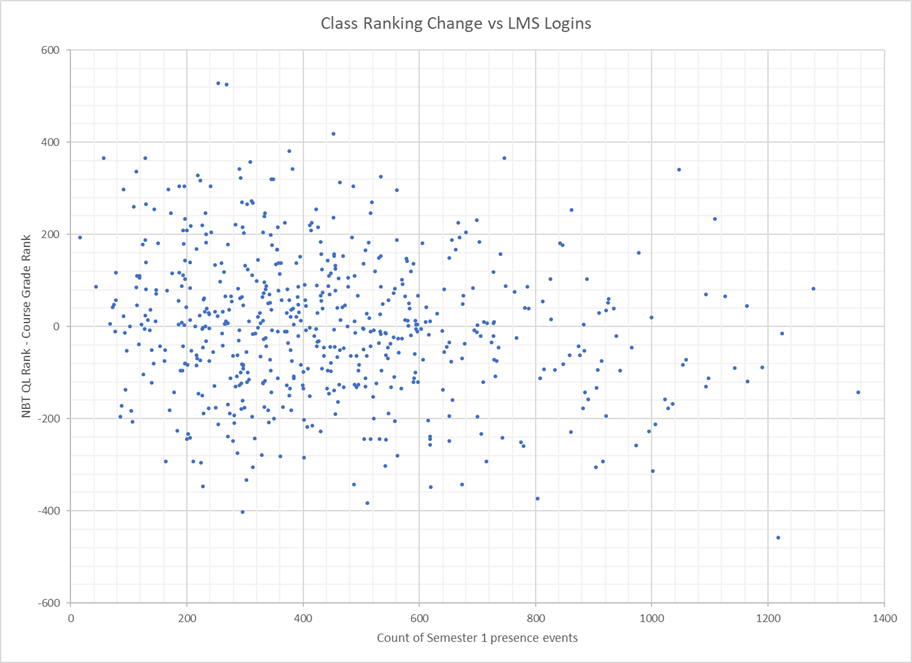
\includegraphics[scale=0.6]{./resources/figures/delta-class-rank.png}
    % \end{mdframed}
    \caption[\( \delta \) class rank vs LMS Logins]{\textbf{Figure \ref{fig-delta-rank}: \( \delta \) class rank vs LMS Logins.} An example of the correlation between \( \delta \) NBT QL ranking scores/course grades compared to LMS usage. As shown in Table \ref{tbl-correlation-variance}, the correlation coefficient between these two datasets is 0.17.}
    \label{fig-delta-rank}
\end{figure}